\section{Geometry Optimization}
% hsolid/11-refine-struct/a-ecut
The molecular structures are optimized in DFT using the vdW-DF functional. We use quantum ESPRESSO v5.3.0 to perform variable-cell geometry optimization at constant pressure. The atomic positions in the optimized unit cell are re-optimized at constant-volume. We use a Troullier-Martins pseudopotential with a core cutoff radius of $r_c=0.5$. The plane-wave cutoff energy is set to 160 Ry. Brillouin zone integration is performed using a shifted Monkhorst-Pack grid with $24^3$, $16^3$, $12^3$ points for the Cmca-4, Cmca-12, and C2/c-24 unit cells, respectively. %The effective number of atoms are 55296, 49152, and 41472, respectively.
Pressure is converged to 0.1 kbar (0.01 GPa). % Forces are converged to

The atomic structure is optimized in DMC. At each density, the $c/a$ parameter determines the I4$_1$/amd-4 ($c/a>1$) crystal structure. To optimize the $c/a$ parameter, we performed 5 DMC calculations at each density. These calculations form a grid in the lattice a-c parameter space as shown in Fig.~\ref{fig:i4-rs-ca}. Please see QMC section for details of the DMC calculations.
\begin{figure}[h]
% 2018-02-01_ani-press
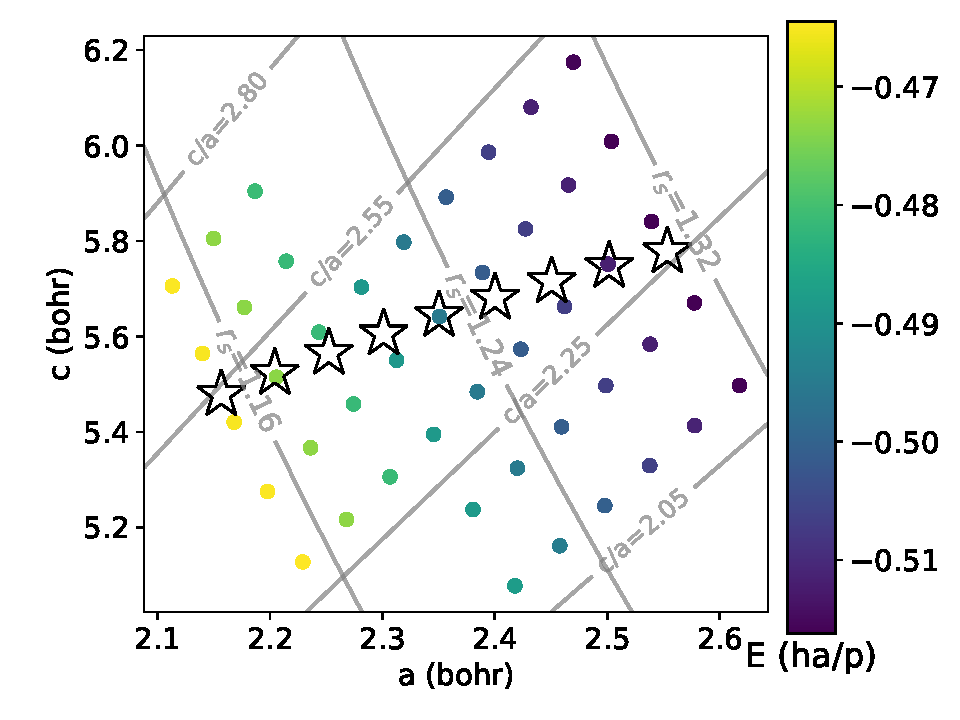
\includegraphics[width=0.8\columnwidth]{70_i4_ca_grid}
\caption{DMC calculations performed to optimize the atomic hydrogen solid structure. Each dot is a structure defined by the lattice parameters a and c. The color of each dot indicates the DMC energy. The gray contour lines mark structures with constant density or c/a ratio. Energy variation is dominated by density change. Energy variation in the c/a direction at fixed density is roughly quadratic around its minimum (black star). The black stars are the optimized geometries.\label{fig:i4-rs-ca}}.
\end{figure}

\section{Relative Enthalpy of Optimized Structures in DFT}
The enthalpies of the optimized crystal structures are calculated in DFT using the vdW-DF functional. As shown in Fig.~\ref{fig:dft-opt-geo},our relative enthalpies agree within 1.5 meV/p with those from McMinis et. al.. Our relative enthalpies for Cmca-12 agree within 1 mha/p with both those from Drummond et. al. and those from McMinis et. al.. Our relative enthalpy for Cmca-4 is higher than that of Drummond by 3.4 mha/p at 400 GPa. % Q/ Is the 3.4 mha/p difference due to structure or functional?
\begin{figure}[h]
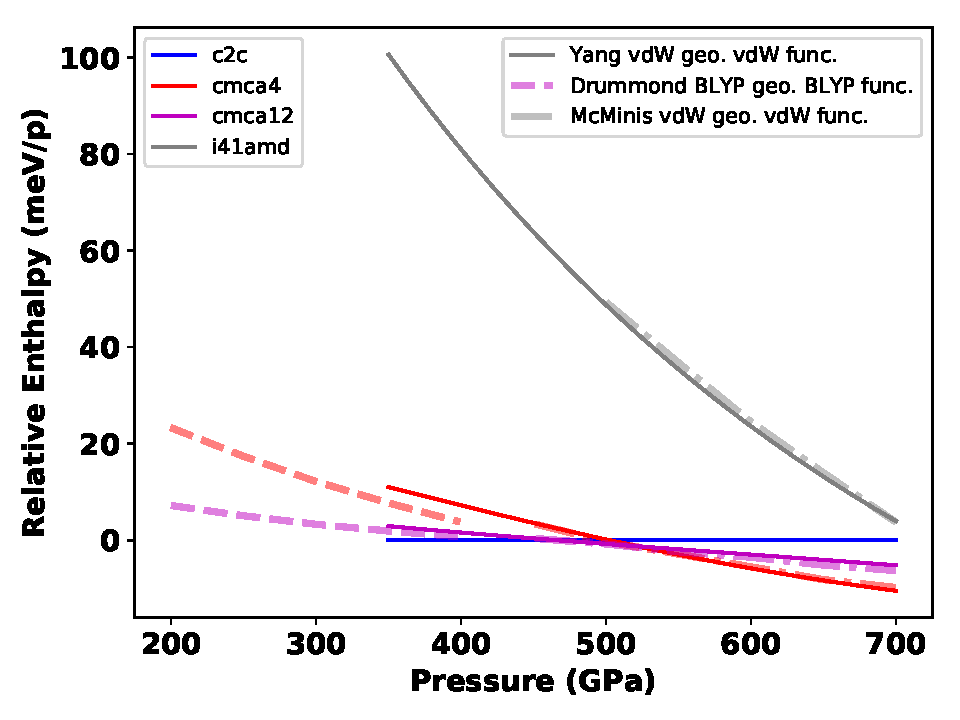
\includegraphics[width=0.8\columnwidth]{010a_dh-vs-p}
\caption{DFT(vdW-DF) enthalpy of optimized structures relative to C2/c-24. Thin solid lines are enthalpies of the Cmca-4, Cmca-12 and I4$_1$/amd using our optimized structures. Dashed lines are DFT(BLYP) enthalpies of Cmca-4 and Cmca-12 from Drummond et. al.. Dash-dot lines are DFT(vdW) enthalpies from McMinis et. al..\label{fig:dft-opt-geo}}
\end{figure}
